\section{Results}\label{sec:results}

SMA-based partitioning of performance observations provides a systematic method for grouping time-correlated performance events.
Once a set of divergence regions has been identified based on crossovers, any number of statistical analyses can be performed on the performance measurements to gain broad but statistically significant correlations between I/O performance and other aspects of the I/O subsystem's utilization and health.
In the following analyses, we separate our 11,986 performance observations into sets of observations that all ran on the same test platform (as described in Table \ref{tab:platform-descriptions}) to characterize the factors that contribute to time-dependent performance variation across different file systems and architectures.

\subsection{Correlative analysis of divergence regions} \label{sec:results/correlate-mira}

\begin{figure}
    \centering
    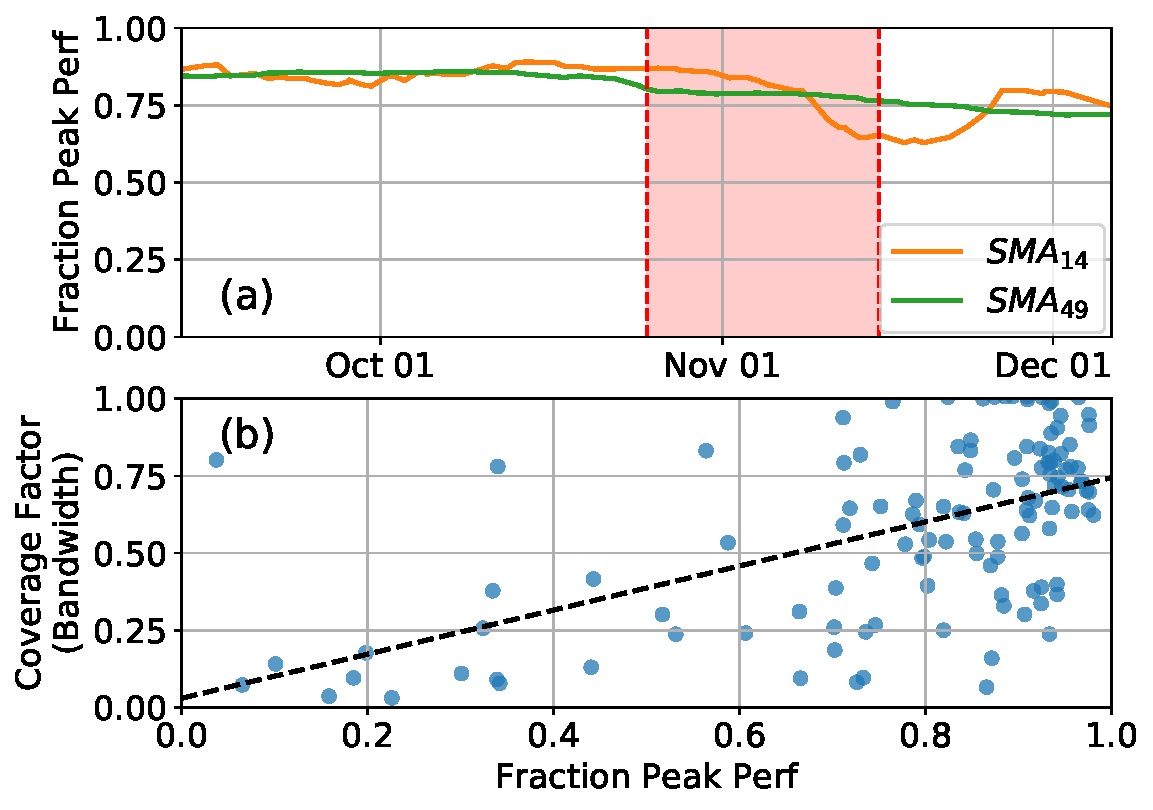
\includegraphics[width=1.0\columnwidth]{mira-correlation-region}
    \vspace{-.35in}
    \caption{Correlation between performance and $CF_{bw}$ in a transition between divergence regions on \mira for all I/O motifs combined.
    (a) shows a region automatically detected using the centroid method, and (b) shows the correlation between performance and $CF_{bw}$ in that region.
    Correlation coefficient is $0.507$ and p-value is ${8.71 \times 10^{-9}}$; dashed line in (b) is a linear fit with slope $0.503$ drawn for visual aid.}
    \label{fig:mira-correlation-region}
    % source: sc18_region-correlation.ipynb
\end{figure}

% Bandwidth, IOPS, and metadata contention are confidently correlated with I/O performance at both long. 

To identify the factors that contribute to time-dependent performance variation, our approach is to apply Pearson correlation to the feature vectors within a divergence region and identify those attributes which correlate with the fraction of peak performance.

Using the entirety of observations generated on \mira \mirafsone as an example, we first calculate ${SMA}_{short}$ and ${SMA}_{long}$ for all benchmark applications and both read and write modes over the year.  
The resulting 34 crossover points define the extents of 33 divergence regions, and one of these regions is depicted in Figure \ref{fig:mira-correlation-region}a.
We then discard all regions that contain fewer than three observations for two reasons:
(a) intuitively, very short divergence regions occur when $\textup{SMA}_{short} \approx \textup{SMA}_{long}$ and there is minimal long-term variation, and
(b) statistically, it is impossible to assert the statistical significance of a correlation with fewer than three data points.
For each of the remaining 32 divergence regions, we then calculate the Pearson correlation coefficients between the fraction of peak performance for each observation and every other attribute in each observation's feature vector.

The result of this process is a new feature vector for each divergence region which contains the correlation coefficients and p-values between the fraction of peak performance and every other attribute across all observations in that region.
Considering only those regions and attributes whose correlations have extremely high significance ($\textup{p-value} < {1.0 \times 10^{-5}}$), we find that nine of the 32 regions exhibit moderate correlation ($R > 0.50$) between performance and any other attribute, and in fact, bandwidth coverage factor is the sole attribute with significant correlation.
The correlation coefficients between performance and bandwidth coverage factor are all moderate to strong, though, and range from 0.507 to 0.884.

The region with the poorest correlation ($R = 0.507$) is shown in Fig. \ref{fig:mira-correlation-region}.
As is evident from the raw data, the relatively poor correlation in this region is due to a cluster of very poorly performing jobs (${0.2 < \textup{fraction peak perf} < 0.4}$) that ran with a relatively high bandwidth coverage factor.
Incidentally, this region is also the single largest divergence region observed on \mira with over 20\% difference between $\textup{SMA}_{short}$ and $\textup{SMA}_{long}$ observed during this time, distinguishing this particular region from the rest of the year.

Despite the unusual region shown in Fig. \ref{fig:mira-correlation-region} though, these data indicate that the time-dependent performance divergences observed on \mira show either moderate or strong coincidence with high degrees of bandwidth contention.
Additionally, this correlation with performance degradation occurs across \emph{all} I/O motifs (similar to Figure \ref{fig:regions-heatmap}a) which distinguishes it from the motif-specific case discussed in Section \ref{sec:features/timedependent}.
The region in Fig. \ref{fig:mira-correlation-region} exhibits a magnitude and relatively modest correlation with bandwidth contention relative to other regions that suggests that some other unmeasured attribute contributed to the observed performance loss.





\subsection{Generalized correlation of time-dependent variation} \label{sec:results/correlate-all}

% - Bandwidth, IOPS, and metadata contention are confidently correlated with I/O performance at both long. 



\begin{figure}
    \centering
    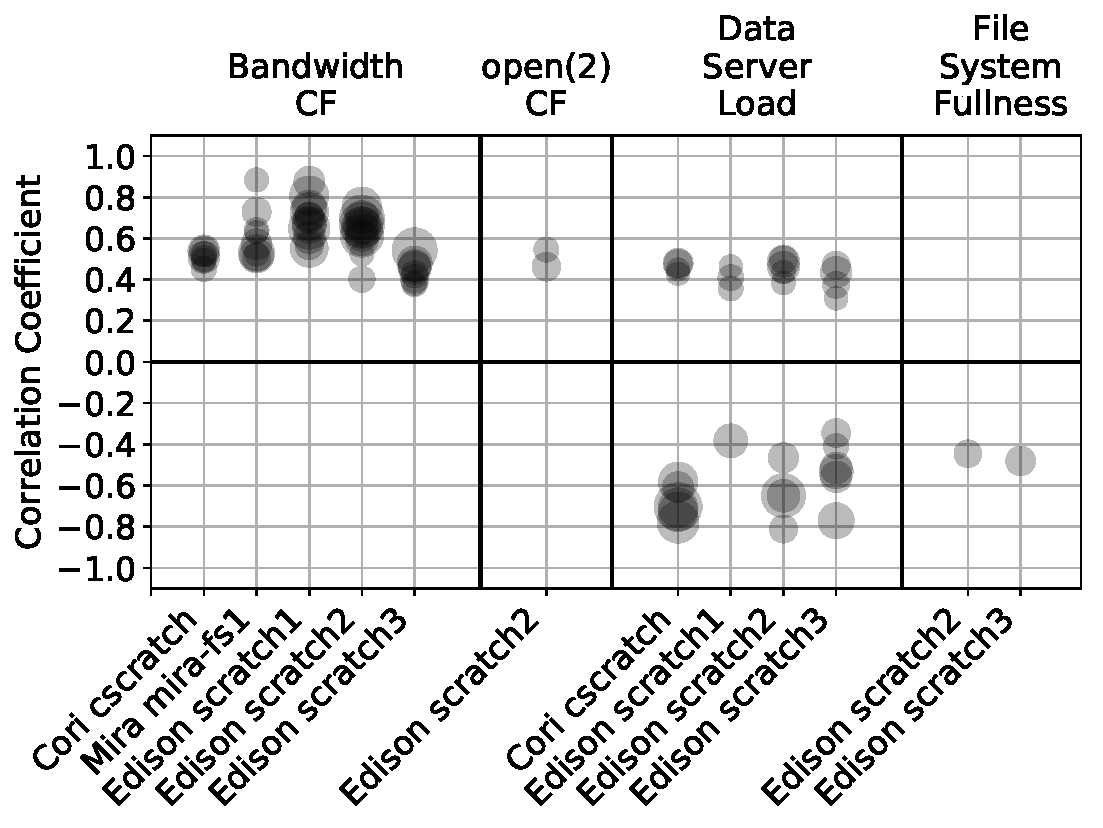
\includegraphics[width=1.0\columnwidth]{trend-correlations}
    \vspace{-.35in}
    \caption{Correlations discovered between fraction peak performance and all other attributes measured during job execution.
    Each circle represents the correlation coefficient over a single trend region, and its diameter is proportional to $-\log_{10}(\textup{p-value}$).
    CF denotes coverage factor.}
    \label{fig:trend-correlations}
    % source: sc18_centroids-allsystems.ipynb
\end{figure}


\begin{figure}
    \centering
    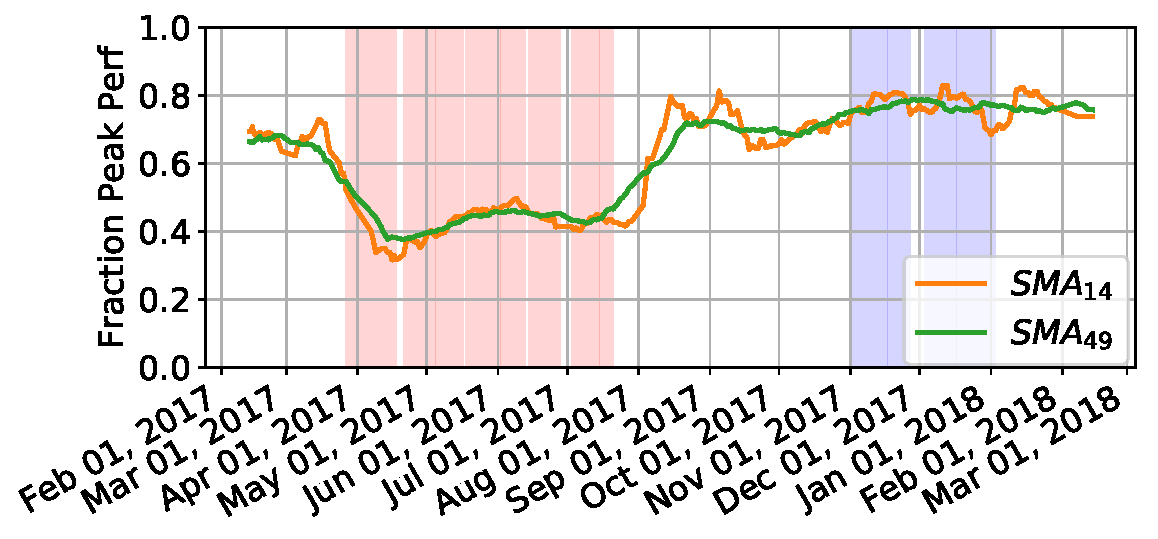
\includegraphics[width=1.0\columnwidth]{cscratch-bimodal-fsaveosscpu}
    \vspace{-.35in}
    \caption{Regions of negative correlation (red) and positive correlation (blue) between fraction peak performance and data server load during trend regions identified on \cori.
    SMAs for \cori's HACC write workload also shown to illustrate the coincidence of a long-term performance issue with the direction of correlation.}
    \label{fig:cscratch-bimodal-fsaveosscpu}
    % source: sc18_centroids-allsystems.ipynb
\end{figure}

Next we apply the same correlation analysis to the other machines in our study, again only keeping correlations with an extremely high significance ($\textup{p-value} < {1.0 \times 10^{-5}}$), and the results of this analysis are shown in Fig. \ref{fig:trend-correlations}.
As was found with Mira in Section \ref{sec:results/correlate-mira}, there is moderate to strong correlation between I/O performance and the bandwidth coverage factor on the Lustre file systems of \cori, and \edison.
Although bandwidth contention resulting in performance loss is intuitive at the scale of a single performance transient, the fact that these correlations were found over longer-term divergence regions indicates that \textbf{bandwidth contention from \emph{sustained workloads} often accompany sustained performance losses}.
This is particularly relevant to the increasing fraction of experimental and observational data that is being processed on modern HPC platforms; as the volume of data being continually streamed from large-scale scientific instruments increases, the effects of sustained bandwidth contention are likely to become increasingly prominent.

% - The sign and magnitude of the correlations changes over time.

Another noteworthy feature that this method reveals is the bimodality of correlation between performance and the CPU load of the file system data servers ("Data Server Load" in Figure \ref{fig:trend-correlations}) on the Lustre-based test platforms.
A time-resolved view of the regions where performance correlates with data server CPU loads (Fig. \ref{fig:cscratch-bimodal-fsaveosscpu}) reveals that the bimodality of the correlation matches the biomodality observed in the HACC write workload on the affected storage systems.
During the long-term performance regression discussed in Section \ref{sec:features/timedependent}, high CPU load on the Lustre OSSs coincided with low performance of the I/O performance probes.
As soon as performance was restored on August 10, the relationship reversed, and high CPU load was observed favorably with respect to performance.
The positive correlation between performance and CPU load is consistent with the data servers using CPUs primarily to service incoming I/O requests, whereas the negative correlation indicates that another CPU load (as may be caused by an algorithmic bug) was present and competed with the data servers' ability to use CPU to service those same requests.
From this, we conclude that not only does baseline I/O performance vary with time, but \textbf{the nature and magnitude of how different attributes correlate with I/O performance also change over time}.
Had this correlation analysis been performed without partitioning over divergence regions, the regions of positive and negative correlation would have obfuscated each other in the net result.

The remaining two attributes that were found to correlate with performance are \texttt{open(2)} coverage factor, which is a measure of metadata resource contention, and file system fullness.
The two divergence regions that demonstrate high metadata coverage factors correlating positively with performance is intuitive, {\color{red}but why was metadata coverage factor so out of whack for so long?}.
% in march 29 case, CF(opens) wasn't high so much as performance was in the toilet
% in nov 26 case,
However, the two instances of file system fullness correlating with negatively with performance occurred at times when their respective file systems approached 90\% full for a period of several days.
The observed loss of performance is consistent with Lustre's known susceptibility to significant performance degradation as OSTs approach 90\% fullness~\cite{oral2014best,Lockwood2017}.

\TODO{Glenn: draw UMAMIs of the metadata rates diagrams to see what's going on.  That result doesn't make any sense.}





\subsection{Transient performance loss} \label{sec:results/shortterm}

\begin{figure}
    \centering
    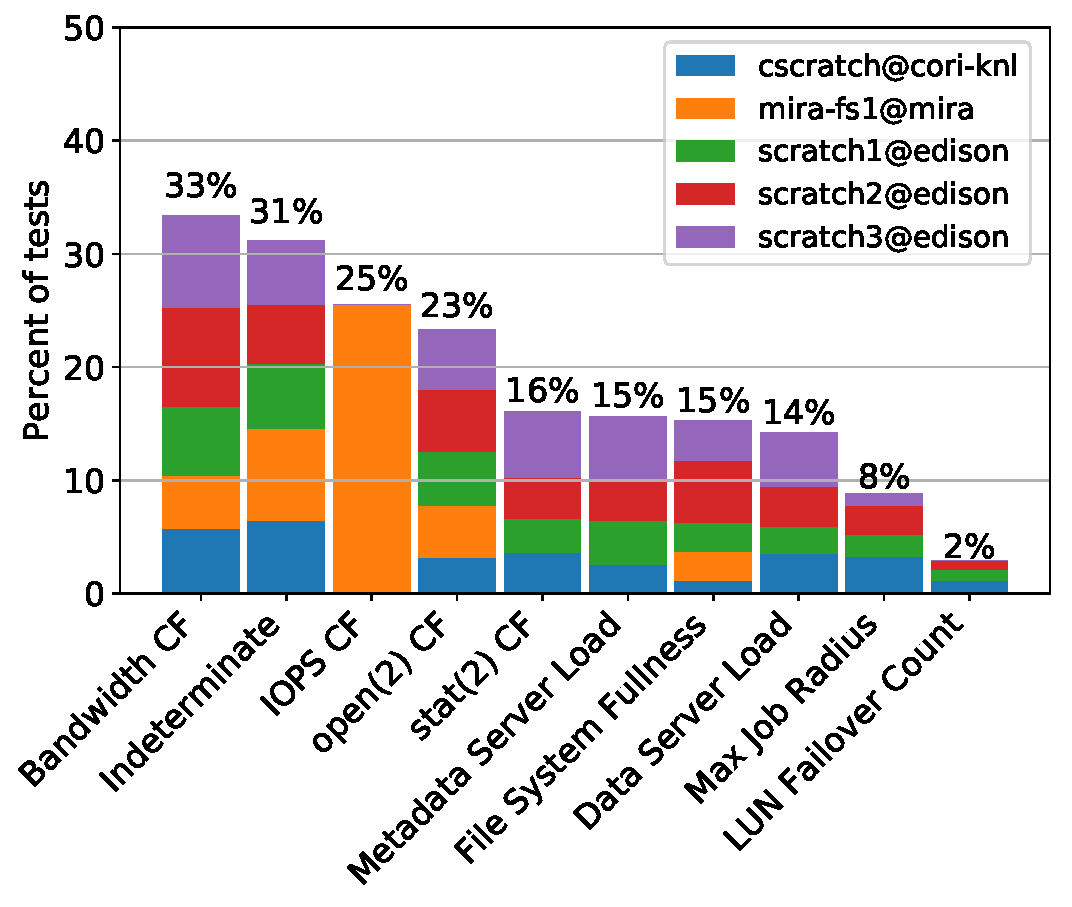
\includegraphics[width=1.0\columnwidth]{contributors-bad-by-system}
    \vspace{-.35in}
    \caption{Attributes that correlated with poor I/O performance across all file systems and benchmarks tested normalized to the number of probes during which each attribute was measured.
    \mira was the only system for which IOPS coverage factor was measured. 
    These data represent 490 anomalous jobs, and 80 jobs (16\%) had no attributes classified as contributors.
    Percentages do not add up to 100\% because multiple attributes are often classified as contributors for a single anomalous job.
    }
    \label{fig:contributors-bad-by-system}
    % source: sc18_umamify-2.0.ipynb
\end{figure}

In addition to characterizing long-term performance issues, it is advantageous to determine the reasons why I/O performance is severely degraded for one and only one day in an otherwise unremarkable period of time.
Such performance losses may only be observed in one of the I/O motifs tested on that day, suggesting a very short-lived issue that disappeared over the course of one or two of the eight daily performance probes.
The lack of a consistent performance trend surrounding these transients makes them difficult to correlate with other metrics as was done in the previous section, a different approach will be required.
Understanding the contributors to these transients is critical to informing the design of storage system hardware and software as well, eventually, mitigating them. 

The performance of a particular performance result (hereafter referred to as the anomalous job) is first contextualized with respect its neighboring jobs, where neighboring jobs are those that
\begin{enumerate}[leftmargin=*]
\item ran in the same period of time, so that we comparing jobs in the same long-term divergence regions, and
\item exhibited the same I/O motif, so we are not comparing jobs whose performance variation may have resulted from having different I/O patterns
\end{enumerate}

In addition to I/O performance, telemetric data collected from other instrumentation sources throughout the I/O subsystem (as described in Section \ref{sec:methods/tokio}) are also associated with each job.
\TODO{How does this work if one jobs spans more than one time point in a telemetric series of data? - NJW}
The anomalous job is then identified as the observation with the worst performance within its divergence region, and any metrics whose worst values were also observed during the anomalous job are classified as possible contributors.
The result is zero or more metrics being flagged as potential contributors to poor performance for each divergence region, application, file system, and read/write mode. For example, if both the performance and the bandwidth coverage factor for the anomalous job are the lowest values observed amongst its neighboring jobs, we classify bandwidth coverage factor as a possible contributor to that poor performance.

%To address these transients, we apply a simple binary classification scheme where metrics are identified as either possible contributors or not.

The statistical significance of these classifications is a function of how many observations are contained in the divergence region where each positive classification is made.
For the sake of setting a limit on uncertainty, we discard all divergence regions whose classifications exceed a p-value of 0.10. \TODO{where is the p-value classification of a divergence region defined ?}
The remaining positive classifications are then grouped by metric and normalized to the number of abnormal jobs where that metric was measured.
The resulting values describe the frequency with which each metric coincides with poor performance across all of the test systems and are shown in Figure \ref{fig:contributors-bad-by-system}.

This analysis reveals that abnormally high contention for bandwidth and IOPS are the metrics that most frequently coincide with abnormally poor performance.
Contention on metadata servers and CPU load on data servers was also observed during anomalous jobs to a less significant degree, consistent with the correlation coefficients shown in Figure \ref{fig:trend-correlations}.
Unlike the correlative analysis, though these data speak directly to the conditions that are present during abnormally poor I/O performance rather than summarize conditions during longer trend periods.
Although the statistical significance of individual metric classifications is relatively high (${\textup{p-value} < 0.10}$), aggregating the classified metrics over all abnormal jobs reveals significantly greater degrees of significance.
For example, the findings shown in Figure \ref{fig:contributors-bad-by-system} all demonstrate p-values of $10^{-4}$ or lower.





\subsection {Discussion}
\label{sec:results/discussion}

\TODO{This is where interesting dribs and drabs are winding up.  Do we carve out a separate section about this stuff, or just drop it?}

Our choice of averaging $\textup{SMA}_{short}$ over ${-0.5w_{short} <= t < +0.5w_{short}}$ makes it insensitive to choice of $w_{short}$.
For the analysis in Section \ref{sec:features/timedependent} changing $\textup{SMA}_{short}$ from $\textup{w}_{14}$ to both $\textup{w}_{7}$ and $\textup{w}_{28}$ resulted in no change to the dates bounding the 139-day divergence region.
The principal effect of changing $\textup{w}_{short}$ is the number of short regions that arise from the higher-frequency oscillations of $\textup{SMA}_{short}$ around $\textup{SMA}_{long}$.

\TODO{This is where a discussion about performance models having to account for long-term changes to baseline performance should go.  That doesn't seem to fit well into the rest of the narrative though.}

We found the exact choice of $w_{short}$ and $w_{long}$ to be somewhat arbitrary; adjusting these values by as much as $\pm 50\%$ did not affect the identification of the most significant events presented here.
In addition, a specific choice of $w$ does not preclude analyzing events longer or shorter than $w$, and we demonstrate methods to address this in Sections XYZ.

Although SMA crossover points are also applied in market analysis for detecting trends in prices and predicting when to buy or sell an asset based on the direction of the crossover~\cite{brock1992simple}.
However, the predictive value of SMA crossovers is a source of controversy even in the financial community, and thus, we focus here solely on using them as tools for detecting trends and partitioning divergent regions in historical datasets.

Financial market analysis techniques can be used to detect underlying trends within noisy I/O performance data.